
\documentclass[10pt, a4paper, twoside]{article}
\usepackage[utf8]{inputenc}
\usepackage{newtxtext,newtxmath} % Times New Roman font
\usepackage[left=2.54cm, right=2.54cm, top=2.54cm, bottom=2.54cm, headheight=15pt]{geometry}
\usepackage{titlesec} % For customizing section titles
\usepackage{enumitem} % Enables bullet points
\usepackage{lipsum} % Add dummy text
\usepackage{hyperref} % Links for references
\usepackage{parskip} % Set spacing between paragraphs
\usepackage{fancyhdr} % Format headers
\usepackage{etoolbox} % Format bibliography header
\usepackage{siunitx} % Used to write SI base units
\usepackage{physics} % Used to write differential equations more easily
\usepackage{graphicx} % Used for figures
\usepackage{caption} % Used to edit the figure captions

% This code is used to supress \qty warning conflict between siunitx and physics packages
\ExplSyntaxOn
\msg_redirect_name:nnn { siunitx } { physics-pkg } { none }
\ExplSyntaxOff

\setlength{\parskip}{10pt}

\titleformat{\section}{\normalfont\fontsize{10}{13}\uppercase}{\thesection.}{1em}{}
\titleformat{\subsection}{\normalfont\fontsize{10}{13}\bfseries}{\thesubsection.}{1em}{}
\titleformat{\subsubsection}{\normalfont\fontsize{10}{13}\itshape}{\thesubsubsection.}{1em}{}

% Redefining \section* command for centered section title
\titleformat{name=\section,numberless}{\normalfont\fontsize{10}{13}\bfseries\centering\uppercase}{}{0pt}{}

% Ensure references title has the same format as \section*
\patchcmd{\thebibliography}{\section*{\refname}}{\section*{REFERENCES}}{}{}

%  Create headers and footers
\fancyhf{} % clear all header and footer fields
\renewcommand{\headrulewidth}{0pt}
\fancyhead[CE]{\fontsize{8}{10}\selectfont \textbf{IAEA-CN-316/2143}}
\fancyhead[CO]{\fontsize{8}{10}\selectfont \textbf{PROKOPYSZYN et al.}}
\fancyfoot[RO]{\fontsize{10}{13}\selectfont \thepage}
\pagestyle{fancy}

% Set the caption font size to 9pt
\DeclareCaptionFont{ninept}{\fontsize{9pt}{12pt}\selectfont}
\renewcommand{\figurename}{\textit{FIG.}}
\captionsetup{
    justification=raggedright,
    singlelinecheck=true,
    font=ninept,
    textfont=it,
    labelfont=it,
    labelsep=period,
    labelformat=simple,
    format=hang
}

\begin{document}
\begin{flushleft}
\fontsize{12}{14}\selectfont \textbf{CONFINEMENT OF FUSION ALPHA-PARTICLES AND ALFV\'EN EIGENMODE STABILITY IN STEP}
% \fontsize{12}{14}\selectfont \textbf{\textit{Subtitle if needed in Times New Roman 12 point bold italic, sentence case}}

\fontsize{10}{13}\selectfont
A.P.K. PROKOPYSZYN, K.G. MCCLEMENTS, H.J.C. OLIVER, M. FITZGERALD, D.A. RYAN, G. XIA \\
United Kingdom Atomic Energy Authority \\
Culham Centre for Fusion Energy, Culham Science Centre, Abingdon, Oxfordshire OX14 3DB, United Kingdom \\
Email: alex.prokopysyzn@ukaea.uk

\end{flushleft}

% Abstract section
\begin{flushleft}
\textbf{Abstract}
\end{flushleft}

\setlength{\parindent}{1cm}
\fontsize{9}{12pt}\selectfont

The Spherical Tokamak for Energy Production (STEP) programme is focused on constructing a fusion power plant prototype that will generate approximately 1.5-1.7 GW of deuterium-tritium fusion energy. To achieve this, the $\alpha$-particles generated through fusion must be adequately confined to maintain the necessary high temperature in the core of the plasma and to protect the wall from too much damage. Microwaves will be used for both external heating and current drive, making $\alpha$-particles the only significant fast-ion species. The purpose of this work is to model the confinement of $\alpha$-particles and the toroidal Alfvén eigenmodes (TAEs) driven by these particles in a variety of scenarios to help determine the best configuration. The scenarios examined here have been identified by the STEP team as potential flat-top operating configurations. We use LOCUST (Lorentz Orbit Code for Use in Stellerators and Tokamaks) to model the $\alpha$-particle confinement and heat-load distribution on the wall, and HALO (HAgis LOcust) to model the TAEs. The results indicate that adequate confinement can be achieved in candidate flat-top operating points, but the results are sensitive to some of the system parameters. For instance, a change in the phase difference between upper and lower edge localised mode (ELM) suppression coils can increase the peak first wall power loading due to $\alpha$-particle losses by a factor of ten.

% Abstract and title over, format text for the main body
\setlength{\parindent}{0pt}
\fontsize{10}{13}\selectfont

\section{Introduction}
\label{sec:introduction}

UKAEA is pioneering efforts to develop a compact prototype of a fusion energy power plant and establish a commercial pathway for fusion energy \cite{nuttall2020, meyer2023, mitchell2023}. A crucial factor in the viability of a deuterium-tritium (D-T) burning fusion reactor is the confinement of fusion-born $\alpha$-particles since, in addition to providing most of the plasma heating, these particles have the potential to damage the reactor walls when unconfined. Ideally, $\alpha$-particles should slow down through Coulomb collisions with thermal electrons and ions while undergoing a modest level of (purely collisional) transport. However, they can drive high-frequency instabilities that may in turn transport them at rates that are well above collisional levels \cite{garcia-munoz2011}. Toroidal Alfv\'en eigenmodes (TAEs) exemplify the type of fast particle-driven instability that can significantly disrupt plasma confinement. In the present work we model $\alpha$-particle losses in the presence of static magnetic fields and determine the stability of TAEs in candidate STEP plasmas with the objective of informing the design process for this device.

External heating and current drive for the plasma in STEP during the flat-top configuration will be provided entirely by microwaves. This heating strategy will utilize a combination of electron cyclotron current drive and electron Bernstein waves. Detailed information on the proposed heating and current drive systems for STEP is provided in \cite{freethy2023}.
This approach has significant implications, as it means that the only substantial population of fast ions will be composed of $\alpha$-particles, which are a product of the fusion reaction itself. Unlike in other tokamak devices such as JET and ITER, STEP will not generate fast ions via neutral beam injectors or ion cyclotron resonance heating systems.
In this context, `fast ions' are defined as ions with speeds that are significantly greater than those of the background plasma, making them `suprathermal'. For example, in the STEP design, the plasma at the core is expected to reach a temperature of approximately 20 keV (see, e.g. \cite{meyer2023,mitchell2023}), whereas the fusion-born $\alpha$-particles will carry an energy of 3.5 MeV, much higher than the background plasma.

For safety and economic reasons, the plasma-facing components (PFCs) must contain the plasma and be highly durable to prevent frequent damage. During operation, the PFCs will be exposed to heat from various sources, even if disruptions are successfully avoided. The wall will be exposed to electromagnetic radiation from the plasma, neutrons, thermal charged particles, runaway electrons, erosion due to sputtering, and $\alpha$-particles. Here, we consider the contribution of $\alpha$-particles. See, for example, \cite{bachmann2018} for a discussion {\it inter alia} of the heat loads on PFCs in a conventional tokamak reactor and \cite{fil2023} for an overview of the modeling of runaway electrons for STEP. Our objective is to maintain the heat load on the wall at a level less than approximately $1\, \text{MWm}^{-2}$ on the first wall of the main chamber, about $5\, \text{MWm}^{-2}$ on dome structures in the divertor regions, and $10\, \text{MWm}^{-2}$ on the divertors themselves. It is important to note that our wall, while incorporating limiters, remains smooth and axisymmetric, although the final design will be comparatively less smooth. Consequently, we must achieve lower heat loads to compensate for shadowing, which can increase the peak heat load.

Because of their large Larmor radii, the confinement of $\alpha$-particles can easily be compromised due to deviations in the background magnetic field from axisymmetry.  In this study, we model $\alpha$-particles in fields that are axisymmetric except for two types of three-dimensional perturbation. The first of these stems from the ripple introduced by the use of a finite number of toroidal field (TF) coils. The second arises from coils that generate resonant magnetic perturbations (RMPs) aimed at suppressing edge-localized modes (ELMs) \cite{zohm1996}.

STEP will need to operate in high-confinement mode (H-mode), and therefore type-I ELMs may pose a significant problem. ELM suppression using RMP coils has been successfully experimentally demonstrated in medium-sized conventional tokamaks such as ASDEX Upgrade \cite{suttrop2018}. However, the nonaxisymmetric RMP fields violate conservation of fast-ion toroidal canonical momentum, and can thus deconfine these ions. The effects of RMPs on fast ions have been studied in DIII-D, ASDEX Upgrade, and ITER \cite{van2015,sanchis2018,ward2022}. Currently, there is no definitive set of criteria for ELM suppression. Therefore, the ELM suppression coils for STEP should be flexible enough to experimentally determine an optimal configuration, and it is necessary to model $\alpha$-particle losses for a range of RMP scenarios.

We only consider the plasma during the flat-top phase as $\alpha$-particle production will be negligible for the greater part of the ramp-up and ramp-down phases. In order to accurately model the $\alpha$-particles we require profiles of temperature and density as well as the magnetic field. These profiles have been determined using the integrated modelling suite JINTRAC \cite{meyer2023, mitchell2023}. This sophisticated tool incorporates a wide range of physics processes, including simplified fast-ion models, providing a comprehensive basis for our analysis.

The structure of this paper is as follows. Section\ref{sec:locust_work} details our efforts using the LOCUST code to model $\alpha$-particle in the flat-top and compute the associated heat load on the wall. In this section, background quantities, such as the magnetic field, are held constant. In Section \ref{sec:halo_work} we consider the magnetic field's response to the presence of $\alpha$-particles and assess TAE stability using the HALO code. In Section \ref{sec:discussion_and_conclusions}, we summarise our findings and discuss their implications.

\section{Alpha particle confinement}
\label{sec:locust_work}

Our goal in this section is to calculate the $\alpha$-particle flux that strikes the walls of STEP and to determine the location and magnitude of the peak flux. To gain a better understanding of how our results are affected by different design choices and parameters, we have run simulations with varying parameters and analysed the particle losses. This analysis is beneficial in the design process, allowing us to identify scenarios that minimise the heat load on the reactor walls.

\subsection{Model}

We calculate the $\alpha$-particle energy flux on the walls of STEP using the LOCUST code (see \cite{akers2018, ward2021} for a more comprehensive explanation of how it works). This tracks particles, represented by markers, which represent samples of the $\alpha$-particle distribution. These markers are traced from birth until they escape and collide with PFCs, or their energy drops below a threshold equal to 1.5 times the bulk ion temperature, at which point they are considered to have thermalised.

We represent the position of the $j^{\text{th}}$ marker at time $t$ by $\mathbf{x}_j(t)$, and denote
the background magnetic field at the position of the marker by $\textbf{B}(\mathbf{x}_j)$.
The forces on the marker due to collisions with the background ions and electrons are $\textbf{F}_{\alpha,i}(\mathbf{x}_j)$ and $\textbf{F}_{\alpha,e}(\mathbf{x}_j)$ respectively, while the mass and charge of the $\alpha$-particles are $m_\alpha$ and $q_\alpha$ respectively. The equation of motion for the $j^{\text{th}}$ marker is
\begin{equation}
m_\alpha\dv[2]{\mathbf{x}_j}{t} = q_\alpha\dv{\mathbf{x}_j}{t}\cross\textbf{B}(\mathbf{x}_j) + \textbf{F}_{\alpha,i}(\mathbf{x}_j) + \textbf{F}_{\alpha,e}(\mathbf{x}_j).
\end{equation}

We do not consider collisions between fast $\alpha$-particles, an omission that is justified by the low concentration of this species, and consequently each $\alpha$-particle is modelled independently. This approach presents substantial computational advantages as it allows for parallel processing. To capitalise on this, LOCUST utilises GPU architecture, enabling the simultaneous modelling of very large numbers of particles. This approach is computationally more efficient and cost-effective than CPU-based modelling. 

We randomly select the initial positions and velocities. The positions are determined by a probability distribution shaped by the Bosch-Hale D-T reaction rate \cite{bosch1992}. We model the birth velocity distribution as isotropic, setting the mean kinetic energy at 3.5 MeV with a spread of about 6\% \cite{brysk1973}. 

We use the most recent design of the first wall for this investigation. The design of the wall, particularly the divertor region, is still being developed, with further iterations expected. The current model does not include details of the eventual design, such as boundaries between the tiles covering the final wall. Our model features a smooth surface, which means that the shadowing effects of the tiles are neglected. The model wall is mainly axisymmetric, but three rows of limiters have been added, eight on the top and bottom rows, and four in the midplane. 

The axisymmetric component of the magnetic field was calculated using the free boundary FIESTA code. This field is generated by the TF and poloidal field (PF) coils, and is modified by the plasma's diamagnetic response. Fig. \ref{fig:lcfs_wall_elm_tf_coils} shows the last closed-flux surface of the axisymmetric field. Additionally, two types of 3D field with a magnitude much smaller than that of the 2D field are included. Despite their small size, these 3D fields can have a large effect on the fast $\alpha$-particle confinement because of their larger gyroradius compared to the bulk plasma ions. Section \ref{sec:tf_ripple_field} models the ripple field produced by the TF coils, and Section \ref{sec:elm_mitigation_field} calculates the impact of the ELM mitigation field on the confinement of the $\alpha$-particles.

At the end of a LOCUST simulation, we calculate the power lost to the inner wall by using the following equation: 
\begin{equation} 
P_{lost} = P_\alpha \frac{\sum_{j\in \text{\{set of markers that hit the wall\}}}\abs{\textbf{v}_{\text{final}, j}^2}}{\sum_{j \in \{\text{set of all markers}\}} \abs{\mathbf{v}_{\text{initial}, j}^2 }}, 
\end{equation}
where $P_\alpha$ is the thermonuclear $\alpha$-particle power, which is equal to $\si{338.MW}$ and is derived from the fusion power. Additionally, $\mathbf{v}_{\text{final}, j}$ is the final velocity of the j\textsuperscript{th} marker upon hitting the wall, and $\mathbf{v}_{\text{initial}, j}$ is the initial velocity of the j\textsuperscript{th} marker after generation by nuclear fusion.

To determine whether PFCs can withstand the impacts of the thermonuclear $\alpha$-particles, we need to know the energy flux of the $\alpha$-particles on the wall. Flux is defined as the flow rate per unit area. The total $\alpha$-particle power across the wall is given by $P_{lost}$, while the $\alpha$-particle energy flux is the power on the wall per unit area and is not evenly distributed across the wall. We calculate the energy flux on the wall using kernel density estimation \cite{chen2017} and leave-one-out cross-validation \cite{chen2017} to determine the bandwidth. We also use bootstrap resampling to calculate 95\% confidence intervals for the maximum $\alpha$-particle energy flux \cite{chen2017}.


\subsection{Results}

\subsubsection{TF ripple field}
\label{sec:tf_ripple_field}

The STEP tokamak is distinguished from conventional tokamaks, such as JET and ITER, by its significant vertical elongation in the $z$-direction. The toroidal field (TF) coils of the current design are projected to be around $\si{22.m}$ tall and have a rectangular shape (see Fig. \ref{fig:lcfs_wall_elm_tf_coils}), although this may be altered in the future. Due to these dimensions, the ripple field induced by the TF coils, represented as $\delta\mathbf{B}^\text{ripple}$, can be aptly approximated by the equation:
% \begin{equation}
%     \label{eq:ripple_field}
%     \begin{aligned}
%         \delta B_R^{\text{ripple}}(R, \phi, z) &= \frac{B_0 R_0}{R} \qty(\frac{R}{R_{\text{coil}}})^{N_{coil}}\sin(N_{\text{coil}}\phi) +  O\qty[\frac{B_0 R_0}{R}\qty(\frac{R}{R_\text{coil}})^{2N_{\text{coil}}}], \\
%         \delta B_\phi^{\text{ripple}}(R, \phi, z) &= \frac{B_0 R_0}{R} \qty(\frac{R}{R_{\text{coil}}})^{N_{coil}}\cos(N_{\text{coil}}\phi)  +  O\qty[\frac{B_0 R_0}{R}\qty(\frac{R}{R_\text{coil}})^{2N_{\text{coil}}}]\\
%         \delta B_z^{\text{ripple}}(R, \phi, z) &= O\qty[\frac{B_0 R_0}{R}\qty(\frac{R}{R_\text{coil}})^{2N_{\text{coil}}}],
%     \end{aligned}
% \end{equation}
\begin{equation}
    \label{eq:ripple_field}
    \begin{aligned}
        \delta B_R^{\text{ripple}}(R, \phi, z) &\approx \frac{B_0 R_0}{R} \qty(\frac{R}{R_{\text{coil}}})^{N_{coil}}\sin(N_{\text{coil}}\phi), \\
        \delta B_\phi^{\text{ripple}}(R, \phi, z) &\approx \frac{B_0 R_0}{R} \qty(\frac{R}{R_{\text{coil}}})^{N_{coil}}\cos(N_{\text{coil}}\phi),\\
        \delta B_z^{\text{ripple}}(R, \phi, z) &\approx 0.
    \end{aligned}
\end{equation}
Here, $R$ denotes the major radius, $R_0$ is the major radius of the plasma's geometric center, $B_0$ represents the toroidal magnetic field when $R=R_0$, $N_{\text{coil}}$ is the count of TF coils, and $\phi$ gives the toroidal angle, expressed in radians. A derivation of Equation \eqref{eq:ripple_field} can be found in, for example, \cite{mcclements2005}.  When we compared Equation \eqref{eq:ripple_field} with the numerical predictions of the ripple field, the discrepancy was below 1\% on the outer side of the plasma. Furthermore, our simulations, using both methodologies, confirmed concordant results within the given statistical error margins (\textbf{make and cite a TDMS here}).

Fig. \ref{fig:max_and_total_flux_vs_rcoil_and_ncoil} shows the maximum energy flux on the walls and the total flux for different radii of the TF coils and the number of TF coils. The current design, with a major radius of approximately $\si{9.m}$ and 16 TF coils, has power losses that remain within acceptable limits. Increasing the design configuration beyond this will have a minimal effect on improving particle confinement from a fast particle perspective. 
% Unfortunately, due to the need to fit other instruments such as the vacuum vessel, it is difficult to reduce the outer radius of the TF coil. The results also show that we can reduce the number of TF coils from 16 to 12 without affecting the confinment (assuming a radius of $9\si{.m}$ is maintained).
Unfortunately, it is difficult to reduce the outer radius of the TF coils due to the need to accommodate other instruments such as the vacuum vessel and PF coils. However, the results indicate that the number of TF coils can be reduced from 16 to 12 without compromising the confinement, provided that the radius of $9\si{.m}$ is maintained.

\begin{figure}[!htb]
    \centering
    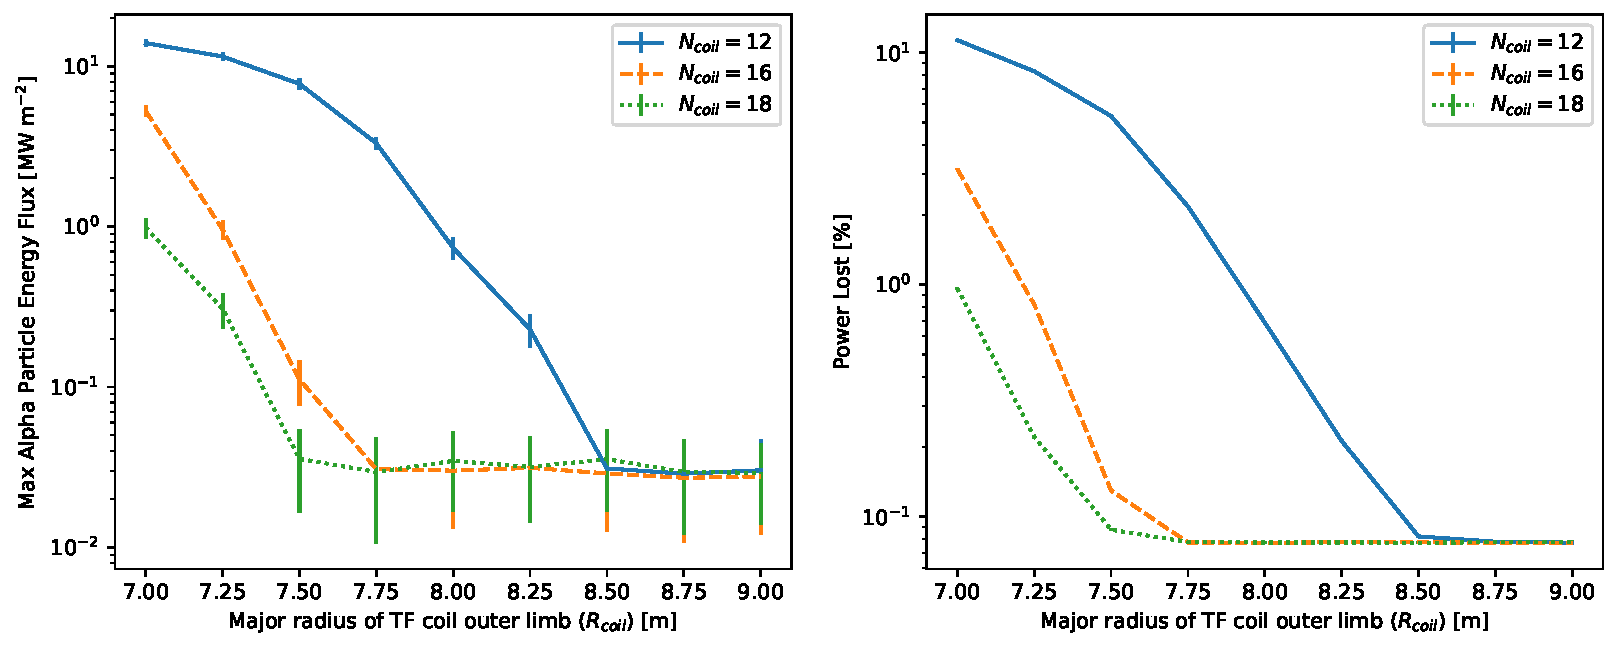
\includegraphics[width=0.99\linewidth]{Figures/max_and_total_flux_vs_rcoil_and_ncoil.pdf}
    \caption{Figure depicts results from 27 simulations. The left column presents the energy flux on the reactor wall, quantified in $\si{MW.m^{-2}}$. The right column indicates the percentage of the $\alpha$-particle power escaping and impacting the plasma facing components. Error bars represent 95\% confidence intervals, reflecting the statistical uncertainty inherent in the Monte Carlo methodology of the simulation.}
    \label{fig:max_and_total_flux_vs_rcoil_and_ncoil}
\end{figure}

\subsubsection{ELM mitigation field}
\label{sec:elm_mitigation_field}

In this section, we will model the confinement of $\alpha$-particles with the ELM mitigation field, excluding the ripple field. The ripple field generated by the most recent TF coil design has a minimal effect on the confinement, so the results presented here are our most accurate estimates of the true confinement of the $\alpha$-particles.

The ELM mitigation field we model is created by the coils shown in Fig. \ref{fig:lcfs_wall_elm_tf_coils}. These coils are located outside the vacuum vessel and are used to generate both the error field correction (EFC) field and the ELM mitigation field. Although it is possible that in the future, resistive wall mode suppression coils located inside the vacuum vessel may be used to generate the ELM mitigation field, the current design prefers to use the EFC coils. Additionally, the number of ELM coils may be altered; at present there are 16 (see Fig. \ref{fig:lcfs_wall_elm_tf_coils}), but this could be reduced to 8.

The current in the $k^\text{th}$ coil, $I_k$, is given by an equation of the form
\begin{equation}
    \label{eq:ELM_coilcurrent_profile}
    I_k = I_0 \cos(n \phi_k + \Delta \phi),
\end{equation}
where $k$ ranges from 1 to 16, $I_0$ is the maximum current value, $\phi_k$ is the toroidal angle of the centre of the $k^\text{th}$ coil, $n$ is the toroidal mode number chosen to be excited, and $\Delta \phi$ is a free parameter that provides a phase shift. This produces a magnetic field that can be expressed as
\begin{equation}
    \delta\textbf{B}^\text{ELM}(R, \phi, z)=\Re\qty[\qty(\delta\textbf{B}^\text{ELM}_\text{real}(R,z) + i\delta\textbf{B}^\text{ELM}_\text{imag}(R,z))\exp[i(n\phi + \Delta \phi)]].
\end{equation}
Other Fourier modes in $\phi$ are present, known as sidebands, but they have a small enough amplitude that their effect on $\alpha$-particle confinement can be disregarded when 16 ELM mitigation coils are used. However, if only 8 coils are employed, the sidebands cannot be ignored \textbf{cite TDMS}.

The ELM mitigation fields create a magnetic field, however, this is altered due to its interaction with the plasma. The plasma's reaction is more prominent for lower toroidal mode numbers ($n$). Therefore, for the ripple field, the plasma's response can be disregarded. For ELM mitigation, we plan to set $n=3$. Greater values of $n$ dissipate more quickly away from the coils, decreasing the power efficiency. Smaller values of $n$ may activate locked modes \cite{ryan2022}. Nevertheless, the decision to use $n=3$ may change and so we will also model the case where $n=2$ and $n=4$. To model the plasma response, we used a code called MARS \cite{liu2015}. It is hard to confirm the accuracy of our plasma response calculations and so we will also analyse the results for the case where the vacuum ELM mitigation field is used.

Equation \ref{eq:ELM_coilcurrent_profile} has three adjustable parameters: the toroidal mode number ($n$), the amplitude ($I_0$), and the phase shift $\Delta \phi$. We will consider the cases where $n$ is equal to 2, 3, and 4. To suppress ELMs, $I_0$ must be large enough, but not so large that it reduces $\alpha$-particle confinement. According to experiments conducted on ASDEX Upgrade, \cite{ryan2022} suggests that for $n=2$, a current of 50 kAt is necessary, for $n=3$ a current of 90 kAt is required, and for $n=4$ a current of 150 kAt is needed. However, there is a high degree of uncertainty over the current needed, so we also model a current with twice these values. Additionally, we investigate the effect of varying the phase shift of the current profile on fast particle confinement. We shall consider $\Delta\phi =$ $0^\circ$, $45^\circ$, $90^\circ$, $135^\circ$, $180^\circ$, $225^\circ$, $270^\circ$, and $315^\circ$.

Fig. \ref{fig:max_and_total_flux_vs_phase} displays the predicted flux of $\alpha$-particle energy on the wall of STEP and the percentage of $\alpha$-power lost, assuming a fusion power of 1.53 GW, which results in a $\alpha$-power of about 304 MW. The results indicate that the results are highly sensitive to the phase shift and a similar phenomenon is observed in \cite{sanchis2018}. Fig. \ref{fig:max_and_total_flux_vs_phase} also shows that the losses are greater when the plasma response to the ELM mitigation field is modelled compared to using the vacuum field. Even when larger current values are used and the plasma response is included, acceptable confinement can be achieved ($<1\si{.MW.m^{^-2}}$) if the right phase shift is chosen. The findings suggest that for $n=3$ and $n=4$, better confinement can be achieved. This could be due to the fact that higher toroidal modes dissipate more rapidly away from the coils, thus reducing the 3D field in the core of the plasma.

\begin{figure}[!htb]
    \centering
    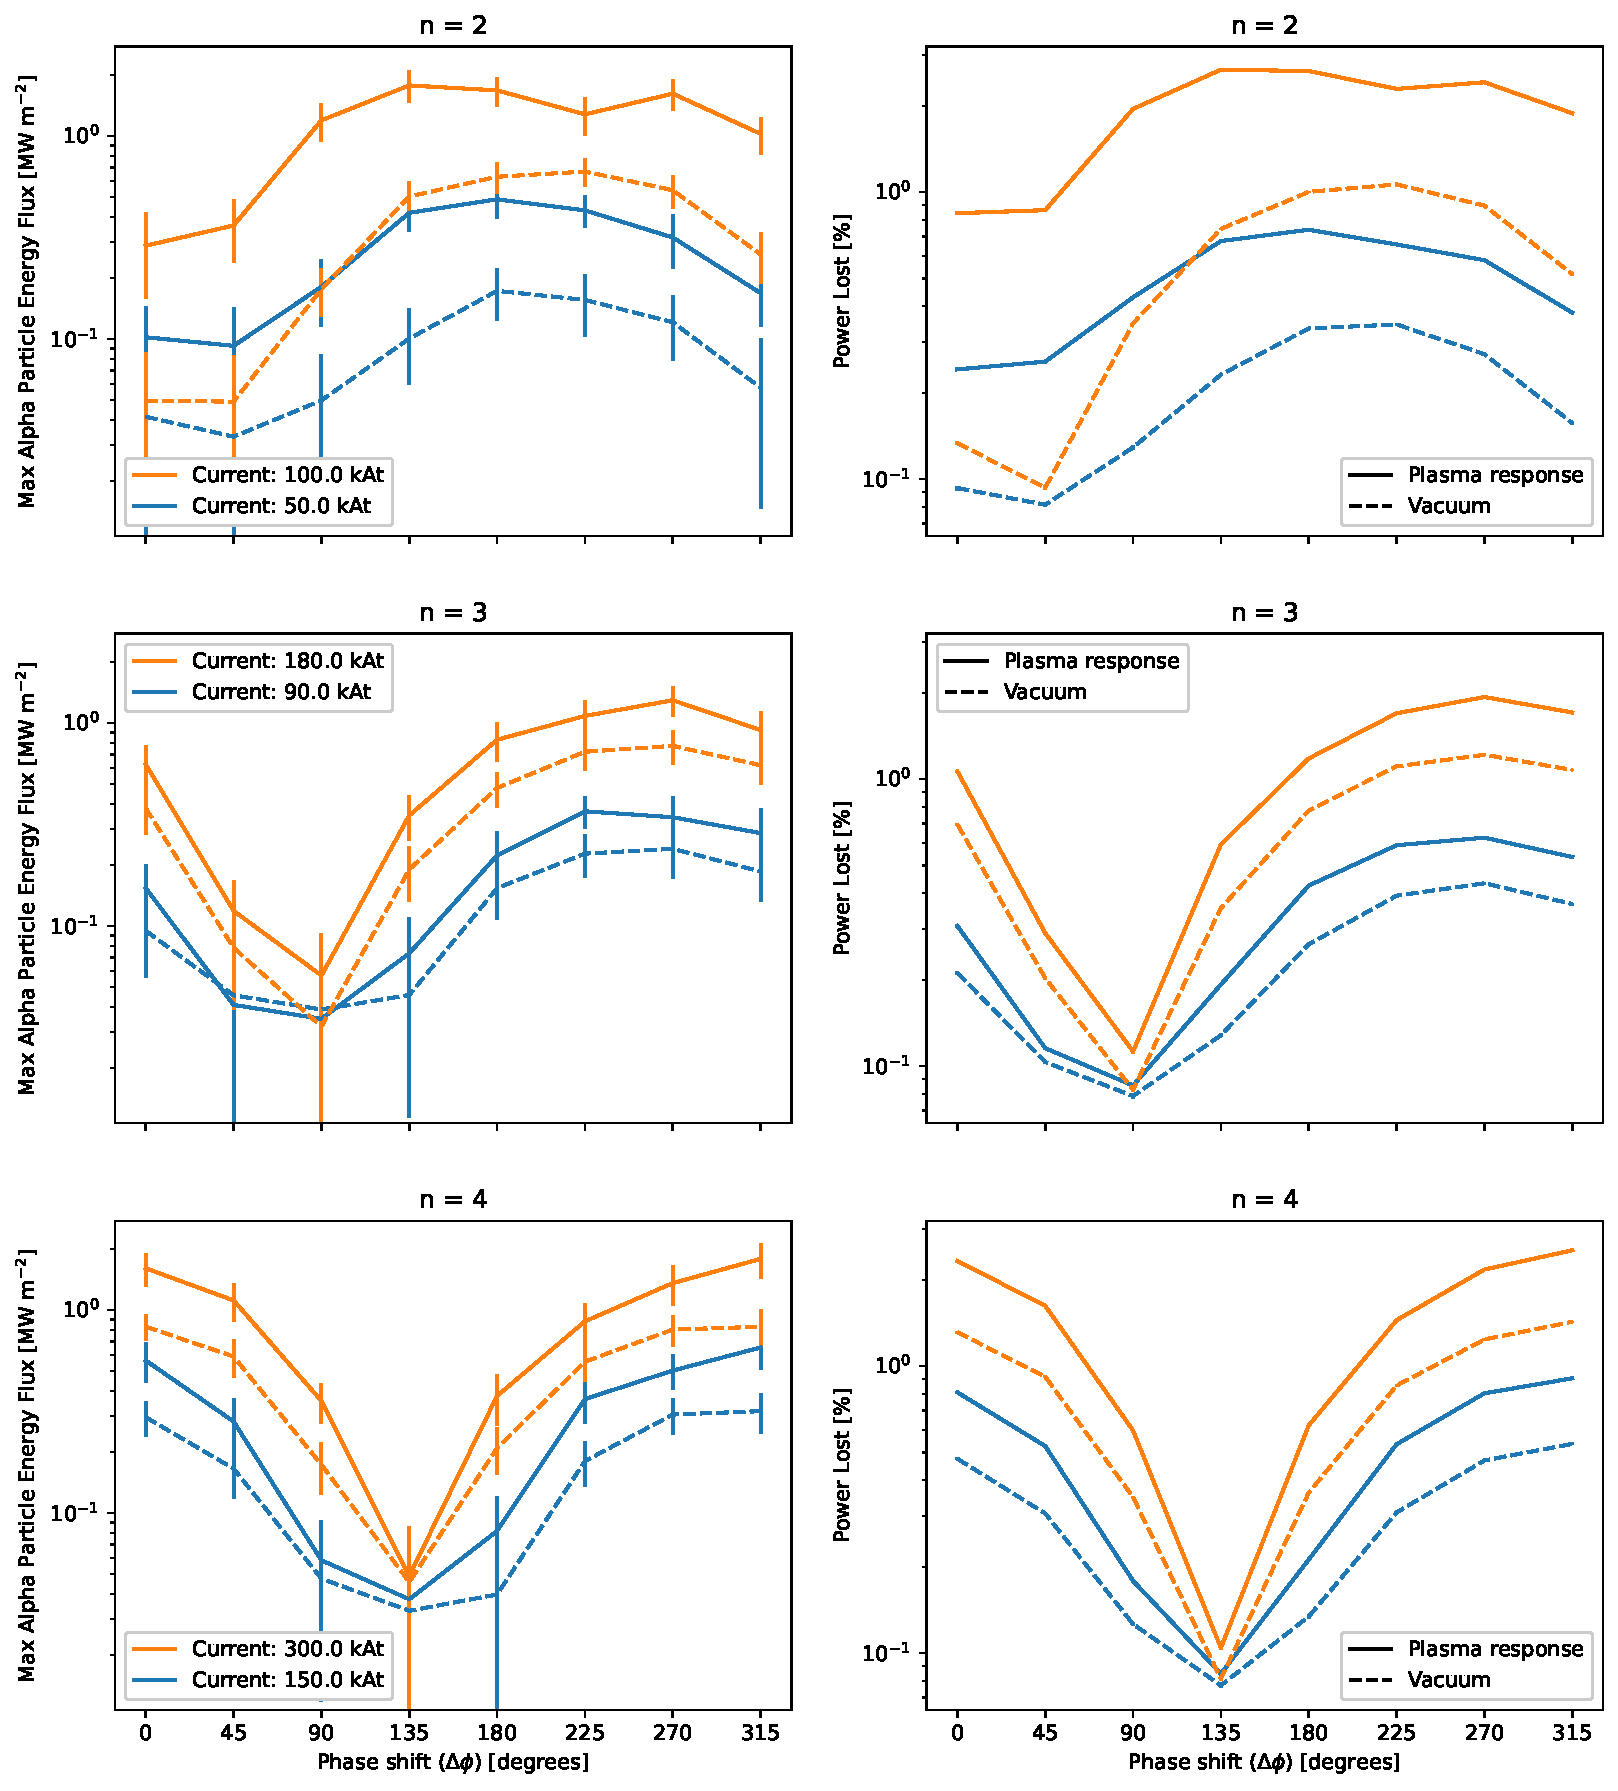
\includegraphics[width=0.99\linewidth]{Figures/max_and_total_flux_vs_phase.pdf}
    % \caption{Caption}
    % \caption{\parbox{0.9\linewidth}{This figure shows the results from 96 simulations. The left-columns s on the wall in $\si{MW.m^{-2}}$}}
    \caption{Figure illustrates outcomes from 96 simulations, comparing $\alpha$-particle losses across different ELM mitigation coil parameters. The column arrangement mirrors that of Fig. \ref{fig:max_and_total_flux_vs_rcoil_and_ncoil}.}
    \label{fig:max_and_total_flux_vs_phase}
\end{figure}

In Fig. \ref{fig:energy_flux_distribution}, we look in more detail at one of the more conservative but likely scenarios where $n=3$, $I_0= 180\si{.kAt}$, $\Delta \phi = 90^\circ$ and where the plasma response is included. More precisely, Fig. \ref{fig:energy_flux_distribution} shows how the $\alpha$-particle energy flux is distributed along the wall. It shows the maximum energy flux of the $\alpha$-particles over all values of $\phi$ as a function of the poloidal distance along the wall ($s_\theta$). Mathematically, it shows
\begin{equation}
    S_{max}(s_\theta) = \max_{0\le \phi \le 2\pi}\qty{S(\phi, s_\theta)},
\end{equation}
where $S=S(\phi, s_\theta)$ denotes the $\alpha$-particle energy flux on the inner wall.
In the right-hand plot of Fig. \ref{fig:energy_flux_distribution}, the boundaries between the outer and inner walls and the upper and lower divertors are marked by vertical lines in blue, orange, green, and red. These are labeled with the symbols +, $\times$, $\bullet$, and $\blacksquare$ respectively. The corresponding symbols and colors are also shown in the left plots for reference.  It shows that the largest peak is on the dome in the upper divertor with another significant peak at the end of the outer leg in the bottom divertor.

\begin{figure}[!htb]
    \centering
    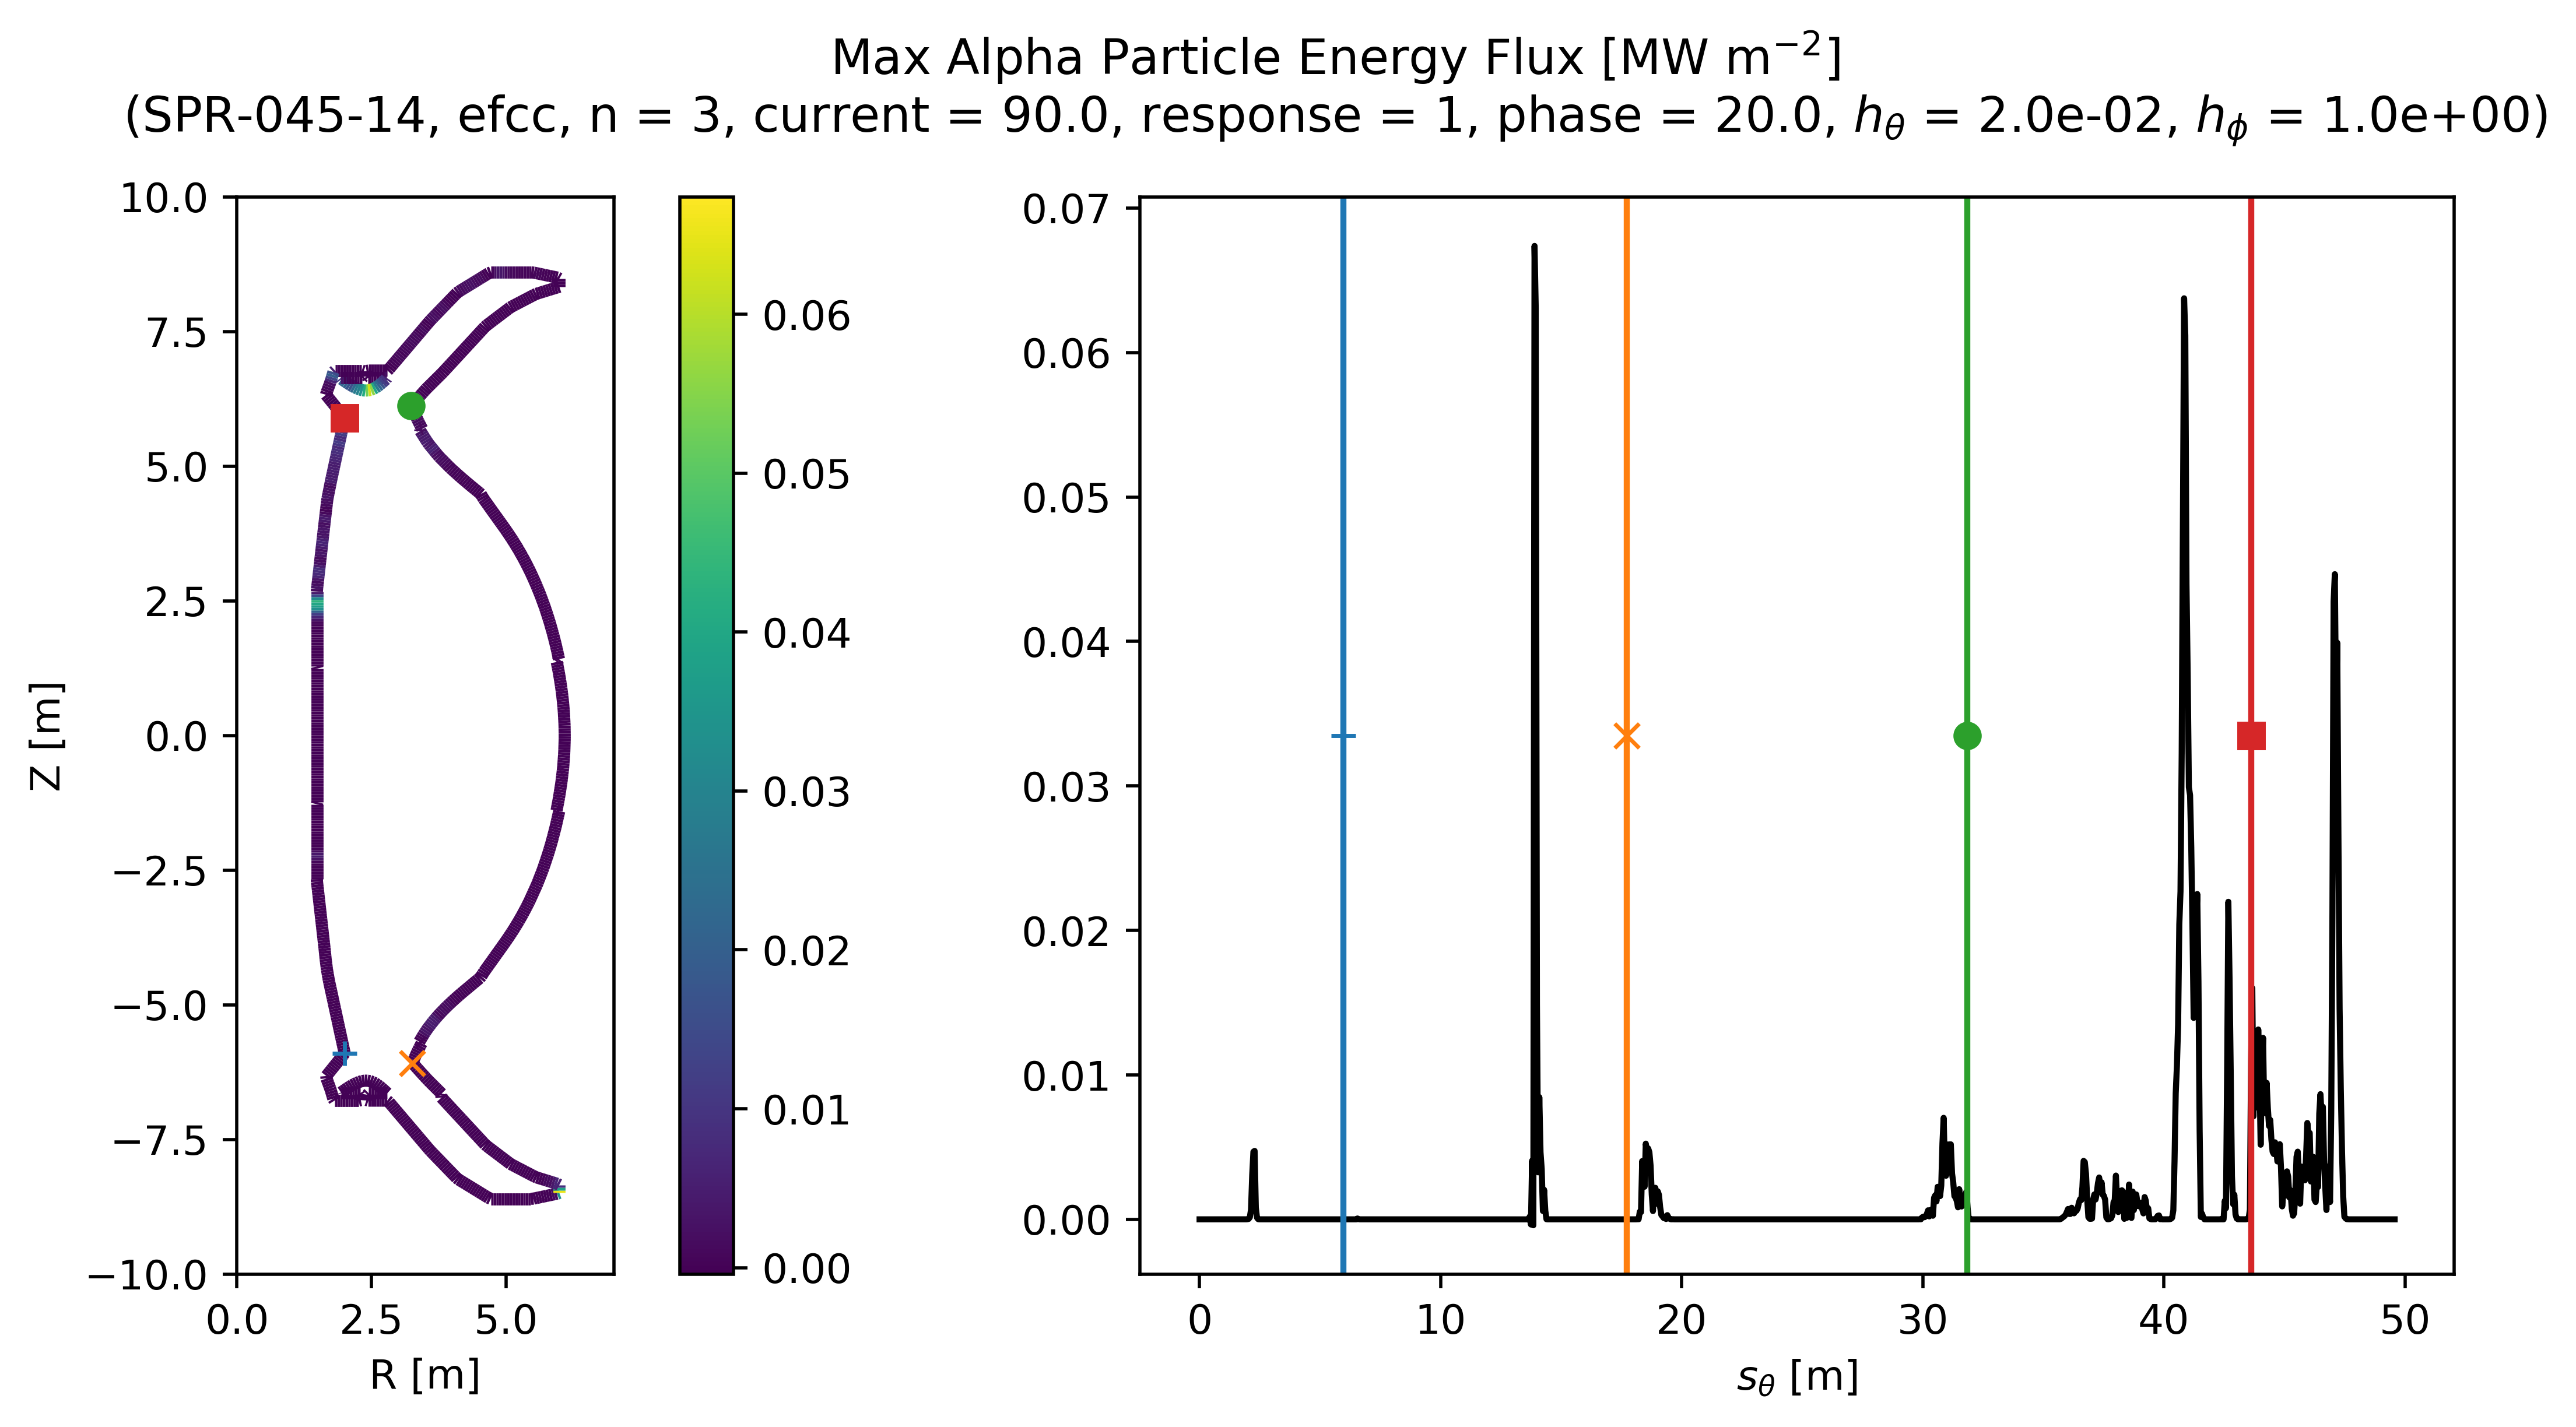
\includegraphics[width=0.7\linewidth]{Figures/simple_line_plot_no_confidence_band.png}
    \caption{This figure illustrates the distribution of the $\alpha$-particle energy flux based on the provided parameters. It depicts the peak $\alpha$-particle energy flux across all $\phi$ values as a function of the poloidal distance, $s_\theta$, along the wall.}
    \label{fig:energy_flux_distribution}
\end{figure}

\section{TAE stability calculations}
\label{sec:halo_work}

\begin{itemize}
    \item MISHKA shows that TAEs exist
    \item However, the growth rate is completely suppressed by the thermal plasma. 
\end{itemize}

\subsection{Model}

\subsection{Results}

\section{Discussion, conclusions and future study}
\label{sec:discussion_and_conclusions}

Our research confirms that, as expected, the confinement of $\alpha$-particles is sufficient in an axisymmetric system. However, this confinement efficiency deteriorates when the ripple field, arising from the use of a finite number of toroidal field (TF) coils, is introduced. Nevertheless, this poses only minor concerns if we opt to position the TF coils inside the vacuum vessel. Given the current plans to locate the TF coils outside the vacuum vessel, with a major radius greater than approximately 9 meters, this is not expected to present significant problems.

The Edge Localised Mode (ELM) mitigation coils pose a more substantial challenge. Our work demonstrates that if the phase between the upper and lower sets of coils is not optimally chosen, it can result in severe deterioration of the confinement of the $\alpha$-particles. Additional research into ELM suppression, particularly for a device with STEP's dimensions, is necessary. Nevertheless, we believe that the work presented here provides valuable insights to inform the design process. This would enable us to find a solution that effectively mitigates the ELMs while also maintaining the acceptable $\alpha$-particle losses.

Resistive Wall Modes (RWMs) are expected to appear in STEP. To address this, we plan to use RWM coils to generate magnetic fields, allowing active and passive control of RWMs, as described in \cite{xia2023}. Since these RWM fields are three-dimensional, there is the potential for a major effect on the confinement of $\alpha$-particles. Our aim is to thoroughly examine the effects of RWM coils on the $\alpha$-particles and to incorporate these results in our comprehensive submission to the Nuclear Fusion journal. We plan to use 8 RWM coils in each row. Therefore, the sidebands, which were discussed in Section \ref{sec:elm_mitigation_field}, will make up a significant part of the RWM field.

In addition to our focus on the flat-top/steady-state phase, as mentioned in Section \ref{sec:introduction}, it is essential to determine if the $\alpha$-particles are adequately confined during the ramp-up and ramp-down phases.

\section*{Acknowledgements}

This work has been funded by STEP, a UKAEA program to design and build a prototype fusion energy plant and a path to commercial fusion.

% Format text for bibliography
% If more than three authors put et al.
\fontsize{9}{12}\selectfont
\setlength{\parskip}{0pt}
\begin{thebibliography}{9}

\bibitem{nuttall2020} % book chapter
% example: CHAPTER-AUTHOR, A., “Title of chapter in sentence case”, Book Title in Title Case, Publisher, Place of Publication (Year).
    WILSON, H., CHAPMAN, I., DENTON, T., et al., 
    ``STEP---on the pathway to fusion commercialization", 
    Commercialising Fusion Energy, 
    IOP Publishing, 
    (2020).

\bibitem{meyer2023} % poster at conference
% example: PRESENTER, A., “Title of presentation in sentence case”, Paper No., paper presented at Organization seminar on subject, Location, year.
    MEYER, H.,
    ``The plasma scenarios for the Spherical Tokamak for Energy Production (STEP) and their technical implications",
    29\textsuperscript{th} IAEA Fusion Energy Conference,
    poster presentation, 
    London, UK, 
    2023

\bibitem{belova2015} % journal article
% example: AUTHOR, A., AUTHOR, B., AUTHOR, C., Journal article title in sentence case, Abb. J. Title 1 2 (Year) 120–123.
    BELOVA, E., GORELENKOV, N., FREDRICKSON, E., et al., 
    Coupling of neutral-beam-driven compressional Alfv\'en eigenmodes to kinetic Alfv\'en waves in NSTX tokamak and energy channeling, 
    Phys. Rev. Lett. 
    \textbf{115} 1 
    (2015) 
    015001.

\bibitem{freethy2023} % poster at conference
% example: PRESENTER, A., “Title of presentation in sentence case”, Paper No., paper presented at Organization seminar on subject, Location, year.
    FREETHY, S.,
    ``The STEP microwave heating and current drive system",
    29\textsuperscript{th} IAEA Fusion Energy Conference,
    poster presentation, 
    London, UK, 
    2023

\bibitem{mitchell2023} % journal article
% example: AUTHOR, A., AUTHOR, B., AUTHOR, C., Journal article title in sentence case, Abb. J. Title 1 2 (Year) 120–123.
    MITCHELL, J., PARROTT, A., CASSON, F., et al.,
    Scenario trajectory optimization and control on STEP,
    Fusion Eng. Des.
    \textbf{192} 
    (2023) 
    113777.

\bibitem{zsolt2023} % internal report
% example: AUTHOR, A., Internal Report Title in Title Case, internal report, Organization, Location, Year.
    ZSOLT, V., et al., 
    TD-001004, 
    internal report, 
    UKAEA, 
    2023.

\bibitem{fil2023} % poster at conference
% example: PRESENTER, A., “Title of presentation in sentence case”, Paper No., paper presented at Organization seminar on subject, Location, year.
    FIL, A., HENDEN, L., NEWTON, S., et al.,
    ``Disruption runaway electron generation and mitigation in the Spherical Tokamak for Energy Production",
    poster presentation, 
    29\textsuperscript{th} IAEA Fusion Energy Conference,
    London, UK, 
    2023

\bibitem{zohm1996} % journal article
% example: AUTHOR, A., AUTHOR, B., AUTHOR, C., Journal article title in sentence case, Abb. J. Title 1 2 (Year) 120–123.
    ZOHM, H., 
    Edge localized modes (ELMs), 
    Plasma Phys. Control. Fusion 
    \textbf{38} 2 
    (1996) 
    105.

\bibitem{wagner1982} % journal article
% example: AUTHOR, A., AUTHOR, B., AUTHOR, C., Journal article title in sentence case, Abb. J. Title 1 2 (Year) 120–123.
    WAGNER, F., BECKER, G., BEHRINGER, K., et al., 
    Regime of improved confinement and high beta in neutral-beam-heated divertor discharges of the ASDEX tokamak, 
    Phys. Rev. Lett. 
    \textbf{49} 19
    (1982) 
    1408.

\bibitem{suttrop2018} % journal article
% example: AUTHOR, A., AUTHOR, B., AUTHOR, C., Journal article title in sentence case, Abb. J. Title 1 2 (Year) 120–123.
    SUTTROP, W., KIRK, A., BOBKOV, V., et al.,
    Experimental conditions to suppress edge localised modes by magnetic perturbations in the ASDEX Upgrade tokamak,
    Nucl. Fusion,
    \textbf{58} 9 
    (2018) 
    096031.
    
\bibitem{van2015} % journal article
% example: AUTHOR, A., AUTHOR, B., AUTHOR, C., Journal article title in sentence case, Abb. J. Title 1 2 (Year) 120–123.
    VAN ZEELAND, M., FERRARO, N., GRIERSON, B., et al.,
    Fast ion transport during applied 3D magnetic perturbations on DIII-D,
    Nucl. Fusion,
    \textbf{55} 7,
    (2015)
    073028.

\bibitem{sanchis2018} % journal article
% example: AUTHOR, A., AUTHOR, B., AUTHOR, C., Journal article title in sentence case, Abb. J. Title 1 2 (Year) 120–123.
    SANCHIS, L., GARCIA-MUNOZ, M., SNICKER, A., et al.,
    Characterisation of the fast-ion edge resonant transport layer induced by 3D perturbative fields in the ASDEX Upgrade tokamak through full orbit simulations,
    Plasma Phys. Control. Fusion,
    \textbf{61} 1,
    (2018)
    014038.
    
\bibitem{ward2022} % journal article
% example: AUTHOR, A., AUTHOR, B., AUTHOR, C., Journal article title in sentence case, Abb. J. Title 1 2 (Year) 120–123.
    WARD, S., AKERS, R., LI, L., et al.,
    LOCUST-GPU predictions of fast-ion transport and power loads due to ELM-control coils in ITER,
    Nucl. Fusion,
    \textbf{62} 12
    (2022)
    126014.

\bibitem{akers2018} % poster at conference
    % example: PRESENTER, A., “Title of presentation in sentence case”, Paper No., paper presented at Organization seminar on subject, Location, year.
    AKERS, R., COLLING, B., HESS, J., et al.,
    ``High fidelity simulations of fast ion power flux driven by 3D field perturbations on ITER",
    poster presentation, 
    26\textsuperscript{th} IAEA Fusion Energy Conference,
    Kyoto, Japan, 
    2016.

\bibitem{ward2021} % journal article
% example: AUTHOR, A., AUTHOR, B., AUTHOR, C., Journal article title in sentence case, Abb. J. Title 1 2 (Year) 120–123.
    WARD, S., AKERS, R., JACOBSEN, A., et al.,
    Verification and validation of the high-performance Lorentz-orbit code for use in stellarators and tokamaks (LOCUST),
    Nucl. Fusion,
    \textbf{61} 8
    (2021)
    086029.

\bibitem{bosch1992} % journal article
% example: AUTHOR, A., AUTHOR, B., AUTHOR, C., Journal article title in sentence case, Abb. J. Title 1 2 (Year) 120–123.
    BOSCH, H., HALE, G.,
    Improved formulas for fusion cross-sections and thermal reactivities,
    Nucl. Fusion,
    \textbf{32} 4
    (1992)
    611-631.

\bibitem{brysk1973} % journal article
% example: AUTHOR, A., AUTHOR, B., AUTHOR, C., Journal article title in sentence case, Abb. J. Title 1 2 (Year) 120–123.
    BRYSK, H.,
    Fusion neutron energies and spectra,
    Plasma Phys.,
    \textbf{15} 7
    (1973)
    611-617.

\bibitem{chen2017} % journal article
% example: AUTHOR, A., AUTHOR, B., AUTHOR, C., Journal article title in sentence case, Abb. J. Title 1 2 (Year) 120–123.
    CHEN, Yen-Chi,
    A tutorial on kernel density estimation and recent advances,
    Biostat. Epidemiol,
    \textbf{1} 1
    (2017)
    161-187.

\bibitem{mcclements2005} % journal article
% example: AUTHOR, A., AUTHOR, B., AUTHOR, C., Journal article title in sentence case, Abb. J. Title 1 2 (Year) 120–123.
    MCCLEMENTS, K.,
    Full orbit computations of ripple-induced fusion $\alpha$-particle losses from burning tokamak plasmas,
    Phys. of Plasmas,
    \textbf{12} 7
    (2005)
    072510.

\bibitem{ryan2022} % internal report
% example: AUTHOR, A., Internal Report Title in Title Case, internal report, Organization, Location, Year.
    RYAN, D., 
    TD-0014685, 
    internal report, 
    UKAEA, 
    2022.

\bibitem{liu2015} % journal article
% example: AUTHOR, A., AUTHOR, B., AUTHOR, C., Journal article title in sentence case, Abb. J. Title 1 2 (Year) 120–123.
    LIU, Y., AKERS, R., CHAPMAN, I., et al.,
    Modelling toroidal rotation damping in ITER due to external 3D fields,
    Nucl. Fusion,
    \textbf{55} 6
    (2015)
    063027.

\bibitem{xia2023} % journal article
% example: AUTHOR, A., AUTHOR, B., AUTHOR, C., Journal article title in sentence case, Abb. J. Title 1 2 (Year) 120–123.
    XIA, G., LIU, Y., HENDER, T., et al.,
    Control of resistive wall modes in the spherical tokamak,
    Nucl. Fusion,
    \textbf{63} 2
    (2023)
    026021.

\end{thebibliography}


\end{document}
